
\def\lfz{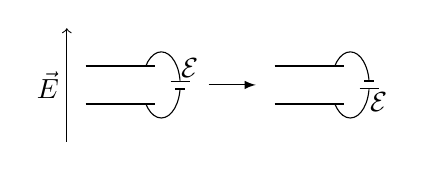
\begin{tikzpicture}[scale=1.2]
  \node at(-.2,0){$\vec E$};
  \draw[->](0,-.6)--(0,.6);
  \draw(1,0) ellipse(.2 and .35);
  \draw[fill=white,white](.2,.2)--(.93,.2)--(.93,-.2)--(.2,-.2)--cycle;
  \draw[thick](.2,.2)--(.93,.2);
  \draw[thick](.2,-.2)--(.93,-.2);
  \draw[fill=white,white](1.1,.04)--(1.3,.04)--(1.25,-.04)--(1.15,-.04)--cycle;
  \draw(1.1,.04)--(1.3,.04);
  \draw[thick](1.15,-.04)--(1.25,-.04);
  \node at (1.3,.18){$\mathcal E$};
  \begin{scope}[xshift=2cm]
  \draw(1,0) ellipse(.2 and .35);
  \draw[fill=white,white](.2,.2)--(.93,.2)--(.93,-.2)--(.2,-.2)--cycle;
  \draw[thick](.2,.2)--(.93,.2);
  \draw[thick](.2,-.2)--(.93,-.2);
  \draw[fill=white,white](1.1,.04)--(1.3,.04)--(1.25,-.04)--(1.15,-.04)--cycle;
  \draw(1.1,-.04)--(1.3,-.04);
  \draw[thick](1.15,.04)--(1.25,.04);
  \node at (1.3,-.18){$\mathcal E$};
\end{scope}
\draw[-latex](1.5,0)--(2,0);
\end{tikzpicture}}

\def\lfd{\begin{tikzpicture}[scale=1.7]
    \tkzDefPoints{0/0/o,0/-2.3/oo,-1.5/-1/a,-1/-1/aa,0/-1.1/c,-.6/-1.1/cc,-1.5/-2/z}
      \tkzDefPoint(240:2.5){b};
      \draw(b)--(o)--(oo);
    \tkzInterLL(a,aa)(o,b) \tkzGetPoint{aaa}
    \draw[postaction={decoration={markings,mark=at position 0.3 with {\arrow{>}}},decorate}
     ](a)--(aaa);
    \tkzDefLine[perpendicular=through aaa,K=.1](o,b)
    \tkzGetPoint{p}
    \tkzDefLine[perpendicular=through aaa,K=-.1](o,b)
    \tkzGetPoint{zp}
    \tkzDefLine[perpendicular=through aaa,K=.1](o,b)
    \tkzGetPoint{azp}
     \tkzDrawLines[add=2 and .3](aaa,p);
    \draw(aaa)--(c)--(cc);
    \tkzDefPointBy[rotation=center c angle 30](aaa)
    \tkzGetPoint{ccc}
    \tkzInterLL(ccc,c)(o,b) \tkzGetPoint{x}
      \draw(x)--(c);
    \tkzDefLine[perpendicular=through x,K=.1](o,b)
    \tkzGetPoint{pp}
    \tkzDefLine[perpendicular=through x,K=-.1](o,b)
    \tkzGetPoint{zpp}
    \tkzDrawLines[add=2 and 1](x,pp);
    \draw[postaction={decoration={markings,mark=at position 0.8 with {\arrow{>}}},decorate}
     ](x)--(z); 
    \tkzDefLine[perpendicular=through x,K=.1](o,oo)
    \tkzGetPoint{ppp}
    \tkzDefLine[perpendicular=through x,K=-.1](o,oo)
    \tkzGetPoint{zppp}
    \tkzDrawLines[add=2.8 and .3](x,ppp);
    \tkzDrawArc[R with nodes](o,.35)(b,oo);
    \node[below=.3,xshift=-3] at(o){\tiny$\varphi$};
%    \tkzDrawArc[red,R with nodes](c,.35)(aaa,cc);
    \tkzDrawArc[R with nodes](aaa,.16)(azp,c);
%    \draw[fill=red](aaa) circle(.01);
%    \draw[fill=red](zp) circle(.01);
%    \draw[fill=red](azp) circle(.01);
    \tkzDrawArc[R with nodes](c,.55)(cc,x);
    \tkzDrawArc[R with nodes](x,.4)(pp,c);
    \tkzDrawArc[R with nodes](x,.3)(zpp,z);
    \tkzDrawArc[R with nodes](x,.5)(zppp,z);
    \tkzDrawArc[R with nodes](aaa,.3)(zp,a);
    \node at(-1.35,-1.6){\tiny$\theta$};
    \node at(-1,-1.45){\tiny$\alpha$};
    \node at(-.8,-.93){\tiny$\varphi$};
    \node at(-.7,-1.8){\tiny$2\varphi{-}\beta$};
    \node at(-.2,-1.4){\tiny$\varphi{-}\beta$};
    \node at(-.3,-.8){\tiny$\beta$};
    \draw[very thin,-latex]((-.65,-1.75)--(-.5,-1.45);
    \draw[very thin,-latex]((-.2,-1.35)--(-.45,-1.15);
    \draw[very thin,-latex]((-.31,-.85)--(-.47,-1.04);
  \end{tikzpicture}}

\def\lfc{\begin{tikzpicture}[scale=1.5]    
    \coordinate (a) at (0, 2.3);
    \tkzDefPoint(295:2.5){b};
    \tkzDefPoint(230:.5){bb};
    \tkzDefPoints{0/0/o,-1/1/c,1/1/d,-.3/-.4/k}
    \draw(0,-.5)--(a);
    \draw (a) -- ++(b);
    \tkzDefPointBy[translation= from o to b](a)
\tkzGetPoint{x}
    \tkzInterLL(a,x)(c,d) \tkzGetPoint{e}
    \draw[postaction={decoration={markings,mark=at position 0.3 with {\arrow{>}}},decorate}
     ](c)--(e);
    \tkzDefLine[perpendicular=through e,K=-.1](a,e)
    \tkzGetPoint{y}
     \tkzDrawLines[add=4.3 and 1](y,e);
    \tkzDefPointBy[translation= from o to bb](e)
\tkzGetPoint{z}
     \tkzInterLL(o,a)(e,z) \tkzGetPoint{u}
     \draw[postaction={decoration={markings,mark=at position .7 with {\arrow{>}}},decorate}
     ](e)--(u);
    \tkzDefLine[perpendicular=through u,K=.3](o,a)
    \tkzGetPoint{w}
     \tkzDrawLines[thin,add=1 and .2](u,w);
    \draw[postaction={decoration={markings,mark=at position .7 with {\arrow{>}}},decorate}
    ](u)--(k);
    \tkzDrawArc[R with nodes](u,.25)(w,k);
    \node[below left] at(u){\tiny$\alpha$};
    \tkzDrawArc[R with nodes](a,.4)(o,e);
    \node[below=.3,xshift=2.5] at(a){\tiny$\varphi$};
    \tkzDrawArc[R with nodes](e,.4)(c,y);
    \tkzDrawArc[R with nodes](e,.33)(y,u);
    \node[below left=.1] at(e){\tiny$\varphi$};
    \node[left=.25,yshift=-3] at(e){\tiny$\varphi$};
\end{tikzpicture}}

\def\lfa{\begin{tikzpicture}
    \def\cA{\begin{tikzpicture}\draw[fill=white](0,0) circle(.13);
        \node at(0,0){A};
      \end{tikzpicture}}
    \def\cV{
\begin{tikzpicture}\draw[fill=white](0,0) circle(.13);
        \node at(0,-.02){V};
      \end{tikzpicture}}
    \draw(3.5,0)--(0,0)--(0,1.3)--(3.5,1.3);
    \draw(1.3,0)--(1.3,1.3);
    \node at(1.3,.65){\cV};
\draw[fill=black](1.3,0) circle(.03);
\draw[fill=black](1.3,1.3) circle(.03);
    \begin{scope}[xshift=25]
    \draw(1.3,0)--(1.3,1.3);
    \node at(1.3,.65){\cV};
\draw[fill=black](1.3,1.3) circle(.03);
\draw[fill=black](1.3,0) circle(.03);
  \end{scope}
  \node at(.65,1.3){\cA};
  \node at(1.75,1.3){\cA};
  \node at(2.65,1.3){\cA};
\draw[fill=black](3.6,0) circle(.03);
\draw[fill=black](3.7,0) circle(.03);
\draw[fill=black](3.8,0) circle(.03);
\draw[fill=black](3.6,1.3) circle(.03);
\draw[fill=black](3.7,1.3) circle(.03);
\draw[fill=black](3.8,1.3) circle(.03);
\draw[white](0,.63)--(0,.7);
\draw[thick](-.15,.7)--(.15,.7);
\draw[thick](-.1,.63)--(.1,.63);
\end{tikzpicture}}

\def\xhref#1#2{\href{#1}{\hskip16pt}\llap{#2}}
\def\xxhref#1#2{\href{#1}{\hskip14pt}\llap{#2}}

\newcommand{\arcangle}{%
  \mathord{<\mspace{-9mu}\mathrel{)}\mspace{2mu}}%
}
\let\arcangle\angle


\def\ora#1{\overrightarrow{#1}}
\def\ee{{\rm{e}}}
\def\e{{\rm{e}}}
\def\F{{\cal F}}
\def\P{{\mathbb{P}}}
\def\Q{{\mathbb{Q}}}
\def\R{{\mathbb{R}}}
\def\Z{{\mathbb{Z}}}
\def\aa{{\bf{a}}}
\def\bb{{\bf{b}}}
\def\cc{{\bf{c}}}
\def\dd{{\bf{d}}}
\def\uu{{\bf{u}}}
\def\vv{{\bf{v}}}
\def\ww{{\bf{w}}}
%\def\C{{\bf{C}}}
\def\e{{\rm{e}}}
\def\WW{{\\cal{W}}}
\def\nwd{{\rm nwd}}
\def\N{\mathbb N}
\def\arctg{\operatorname{arc\,tg}}
\def\arcctg{\operatorname{arc\,ctg}}
\def\xx{{\bf x}}
\def\bb{{\bf b}}
\def\sqqrt#1{\sqrt{\vphantom{b}\smash{#1}}}
\def\bdot{\mathop{\lower-2pt\hbox{\bf.}}}
\def\sqqrt#1{\sqrt{\vphantom{b}\smash{#1}}}

\def\frac#1#2{{#1\over#2}}

\long\def\zad#1#2#3#4{\par Zadanie {\bf#1.} [#4] ($WT$~=~#2;
$LPR$~=~#3).}


\def\Ada{{\bf Michał Adamaszek}}
\def\ada{{\bf M.~Adamaszek}}
\def\Bed{{\bf Witold Bednarek}}
\def\bed{{\bf W.~Bednarek}}
\def\bes{{\bf S.~Bednarek}}
\def\Cis{{\bf Jerzy Cisło}}
\def\cis{{\bf J.~Cisło}}
\def\Dan{{\bf Andrzej Daniluk}}
\def\dan{{\bf A.~Daniluk}}
\def\Fie{{\bf Janusz Fiett}}
\def\fie{{\bf J.~Fiett}}
\def\Kam{{\bf Krzysztof Kamiński}}
\def\kam{{\bf K.~Kamiński}}
\def\Kas{{\bf Marcin Kasperski}}
\def\kas{{\bf M.~Kasperski}}
\def\Kit{{\bf Szymon~Kitowski}}
\def\kit{{\bf S.~Kitowski}}
\def\Kna{{\bf Bartłomiej~Knapik}}
\def\kna{{\bf B.~Knapik}}
\def\Kub{{\bf Paweł Kubit}}
\def\kub{{\bf P.~Kubit}}
\def\Kuj{{\bf Radosław Kujawa}}
\def\kuj{{\bf R.~Kujawa}}
\def\Kum{{\bf Piotr Kumor}}
\def\kum{{\bf P.~Kumor}}
\def\Kur{{\bf Andrzej Kurach}}
\def\kur{{\bf A.~Kurach}}
\def\Kwi{{\bf Miłosz Kwiatkowski}}
\def\Lab{{\bf Paweł Łabędzki}}
\def\lab{{\bf P.~Łabędzki}}
\def\Maz{{\bf Krzysztof Maziarz}}
\def\maz{{\bf K.~Maziarz}}
\def\mor{{\bf K.~Morawski}}
\def\Mro{{\bf Barbara Mroczek}}
\def\mro{{\bf B.~Mroczek}}
\def\Naj{{\bf Paweł Najman}}
\def\naj{{\bf P.~Najman}}
\def\Ols{{\bf Janusz Olszewski}}
\def\ols{{\bf J.~Olszewski}}
\def\Ord{{\bf Tomasz Ordowski}}
\def\ord{{\bf T.~Ordowski}}
\def\Pat{{\bf Mikołaj Pater}}
\def\pat{{\bf M.~Pater}}
\def\por{{\bf N.~Porwol}}
\def\ska{{\bf Z.~Skalik}}
\def\Spy{{\bf Marek Spychała}}
\def\spy{{\bf M.~Spychała}}
\def\Tur{{\bf Szymon~Tur}}
\def\tur{{\bf S.~Tur}}
\def\War{{\bf Michał Warmuz}}
\def\war{{\bf M.~Warmuz}}
\def\Weg{{\bf Jakub Węgrecki}}
\def\weg{{\bf J.~Węgrecki}}
\def\Wie{{\bf Tomasz Wietecha}}
\def\wie{{\bf T.~Wietecha}}
\def\Wis{{\bf Piotr Wiśniewski}}
\def\wis{{\bf P.~Wiśniewski}}
\def\Wor{{\bf Adam Woryna}}
\def\wor{{\bf A.~Woryna}}
\def\Zyg{{\bf Krzysztof Zygan}}
\def\zyg{{\bf K.~Zygan}}
\def\Zmi{{\bf Bartłomiej Żmija}}
\def\zmi{{\bf B.~Żmija}}




\setcounter{equation}0
\normalsize

%\makeatletter
%\def\@oddhead{\hbox to\hsize{\kern-7.5cm\rlap{\color{magenta!20}{\vrule height.9cm depth-1mm width22.5cm}}\kern2cm{\textcolor{white}{\LARGE\raise3mm\hbox{\textsf{\textbf{Liga zadaniowa Wydziału Matematyki, Informatyki i~Mechaniki,}}}}\hfill}\hfill\kern-3cm}}\makeatother

% LIGA--MATEMATYCZNA--ZDEFINIOWANIE
\ligaspis
\long\def\matematyka{ 
%\vspace{-30pt}
%\baselineskip11.7pt plus.3pt minus.2pt 
\klub[15]{m}
  \Magenta{\textbf{Zadania z~matematyki nr 895, 896}}%
  \marg[10]{Termin nadsyłania rozwiązań: \rlap{30 IV 2025}\medskip

\long\def\nic##1{}\nic{
{\centering
Czołówka ligi zadaniowej {\bf Klub 44~M}\\
po uwzględnieniu ocen rozwiązań
zadań 841 ($WT=1{,}42$) i~842 ($WT=2{,}98$)
z~numeru 5/2022
\vskip2pt}\tabcolsep5.5pt
\begin{tabular}{@{}llr}
Jerzy Cisło& Wrocław &43,97\\
Krzysztof Maziarz &Kraków &40,67\\
Stanisław Bednarek&Łódź &38,92\\
Paweł Najman&Kraków &38,88\\
Marcin Kasperski&Warszawa &37,65\\
Tomasz Wietecha&Tarnów &37,64\\
Krzysztof Zygan&Lubin &36,17\\
Adam Woryna&Ruda Śl. &36,14\\
Mikołaj Pater&Opole &34,62\\
Radosław Kujawa&Wrocław &33,74\\
Norbert Porwol&Essen &32,73\\
\end{tabular}}
}

\Black{\textit{Redaguje Marcin E. KUCZMA}}


{\bf895.}
Na okręgu zaznaczono $n$ punktów; ${n\ge3}$ jest ustaloną liczbą nieparzystą. Każdemu punktowi została przyporządkowana wartość 0 lub~1. Dozwolone są ruchy polegające na wybraniu trzech kolejnych punktów o~wartościach (kolejno) $a,b,c$ takich, że ${a=c}$, i~zamianie $b$ na~$1{-}b$. Udowodnić, że startując z~dowolnej konfiguracji i~wykonując dozwolone ruchy, można uzyskać jednakową wartość dla wszystkich $n$ punktów.

{\bf896.}
Udowodnić, że ciąg $(A_1,A_2,A_3,\ldots)$ o~wyrazach
$$
 A_n=\frac1n\sum\limits_{k=1}^{2^n}\frac1k
$$
jest malejący.

\textit{Zadanie 896 zaproponował pan Jerzy Cisło z~Wrocławia}

%\vspace*{\parskip}
%\vskip16pt

\marg[-80]{
{\centering

    Lista uczestników ligi zadaniowej\kern27pt

    {\bf Klub~44~M}\kern27pt

    po zakończeniu sezonu\kern27pt

    (roku~szkolnego)~2023\slash24\kern27pt

}\smallskip
\vbox{\halign{##\hfil~~&~~\hfil##\cr
Szymon Kitowski      &     41,11\cr
Witold Bednarek      &  9--40,58\cr
Mikołaj Pater       &  3--39,58\cr
Krzysztof Zygan      &  1--39,38\cr
Tomasz Wietecha      & 14--38,61\cr
Andrzej Daniluk      &  2--37,89\cr
Szymon Tur           &     35,35\cr
Andrzej Kurach       &  3--33,24\cr
Jędrzej Biedrzycki  &     32,29\cr
Krzysztof Kamiński  &  3--30,48\cr
Marian Łupieżowiec &  1--29,87\cr
Michał Warmuz       &     29,84\cr
Marcin Kasperski     &  5--28,94\cr
Marcin Małogrosz    &  4--27,82\cr
Roksana Słowik      &  2--27,60\cr
Janusz Olszewski     & 24--26,40\cr
Janusz Wojtal        &     26,30\cr
Grzegorz Wiączkowski&     26,13\cr
Błażej Żmija      &  2--25,48\cr
Maciej Mostowski     &  1--22,90\cr
Krzysztof Maziarz    &  1--22,58\cr
Stanisław Bednarek  &  3--22,47\cr
Marek Spychała      &  5--22,32\cr
Piotr Wiśniewski    &  1--20,59\cr
Barbara Mroczek      &     18,58\cr
Grzegorz Karpowicz   &  2--17,76\cr
Jerzy Cisło         & 17--17,54\cr
Patryk Jaśniewski   &  1--16,62\cr
Piotr Łaba          &     14,50\cr
Zbigniew Skalik      &  4--12,48\cr
Paweł Łabędzki    &  1--12,47\cr
 }}
\smallskip

Legenda (przykładowo):\\ stan konta 9--40,58 oznacza, że uczestnik
już dziewięciokrotnie zdobył 44~punkty, a~w~kolejnej (dziesiątej)
rundzie ma 40,58~punktów.

\smallskip
Zestawienie obejmuje wszystkich uczestników ligi, którzy
spełniają następujące dwa warunki:

-- stan ich konta (w~aktualnie wykonywanej rundzie) wynosi co
najmniej 12~punktów;

-- przysłali rozwiązanie co najmniej jednego zadania z~rocznika
2022, 2023 lub~2024.

\smallskip

Nie drukujemy więc nazwisk tych uczestników, którzy rozstali
się z~ligą trzy lata temu (lub dawniej); oczywiście jeśli
ktokolwiek z~nich zdecyduje się wrócić do naszych
matematycznych łamigłówek, jego nazwisko automatycznie wróci
na listę. Serdecznie zapraszamy!
\smallskip
}\Magenta{\textbf{Rozwiązania zadań z~numeru 10\slash2024}}

\Magenta{
{\footnotesize Przypominamy treść zadań:}

{\scriptsize
   

{\bf887.}
Znaleźć najmniejszą liczbę rzeczywistą~$A$, dla której istnieją liczby zespolone~$u,v,w$ oraz liczba rzeczywista~$B$ takie, że ${|u|=|v|=|w|=1=uvw}$, zaś ${u+v+w=A+Bi}$.


{\bf888.}
Znaleźć wszystkie trójki liczb całkowitych ${x,y,z\ge0}$ spełniające równanie \ ${7^x+2^{x+y}=z^2}$.

}
}


\smallskip

%\advance\baselineskip by-.3pt
{\bf887.}
Prościej: chodzi o~wyznaczenie minimalnej wartości
${{\rm{Re}}(u+v+w)}$ dla liczb $u,v,w$ o~podanych własnościach. Są to liczby o~module~1, zatem istnieją liczby rzeczywiste $x,y,z$ takie, że
${u=\ee^{ix}}$,
${v=\ee^{iy}}$,
${w=\ee^{iz}}$.
Warunek ${uvw=1}$ oznacza, że ${x+y+z=2k\pi}$ (${k\in\Z}$). Przy tym
$$
{\rm{Re}}(u+v+w)={\rm{Re}}(u)+{\rm{Re}}(v)+{\rm{Re}}(w)=\cos{x}+\cos{y}+\cos{z}.
$$
Należy znaleźć minimum tej sumy przy powyższym warunku.

Niech ${c=\cos\frac{x+y}2}$; \ więc \ ${\cos{x}+\cos{y}=2\cos\frac{x+y}2\cos\frac{x-y}2\ge-2|c|}$; \ a~skoro ${z=2k\pi-(x+y)}$, zatem \
${\cos{z}=\cos\bigl(2\cdot\frac{x+y}2\bigr)=2c^2-1}$. \ W~konsekwencji
$$
\textstyle
\cos{x}+\cos{y}+\cos{z}\ge2c^2-2|c|-1=2\bigl(|c|-\frac12\bigr)^2-\frac32\ge-\frac32\,.
$$
W~tych szacowaniach zachodzi równość, gdy ${x=y=z=\pm\frac23\pi}$ (co odpowiada liczbom ${u=v=w=\cos(\frac23\pi)\pm{i\,\sin(\frac23\pi)}}\,$). Szukane minimum wynosi więc~$-\frac32$.


\medskip
{\bf888.}
Niech liczby ${x,y\ge0}$, ${z>0}$ spełniają zadane równanie. Gdy ${x=0}$, wtedy ${2^y=(z-1)(z+1)}$, więc ${z\pm1}$ to potęgi dwójki, skąd ${z=3}$ i~${y=3}$. Trójka $(0,3,3)$ jest jednym z~rozwiązań.

Gdy ${x=1}$, równanie ma postać \ ${7+2^{y+1}=z^2}$, \ więc $z$ jest liczbą nieparzystą. Dostajemy ${2^{y+1}\equiv2}$~(mod~4), czyli ${y=0}$; wtedy ${z=3}$. Trójka $(1,0,3)$ jest jednym z~rozwiązań.

Dalej rozważamy ${x\ge2}$. Dane równanie pokazuje, że ${3^x\equiv{z^2}}$~(mod~4), co jest możliwe tylko dla parzystego~$x$. Niech więc ${x=2t}$ (${t\ge1}$); zapiszmy równanie tak: \ ${(z+7^t)(z-7^t)=2^{2t+y}}$. \ Pierwszy czynnik po lewej stronie jest liczbą dodatnią, więc drugi też; stąd ${z\ge8}$. Oba czynniki muszą być potęgami dwójki:
$$
z+7^t=2^k,\quad z-7^t=2^l\quad (k>l\ge0,\;\;k+l=2t+y).
$$
Po odjęciu stronami: \ ${2\cdot7^t=2^l(2^{k-l}-1)}$, skąd ${l=1}$, ${7^t=2^{k-1}-1}$.

\looseness-1 {\spaceskip.33em minus.1emGdy $k=4$, dostajemy $t=1$ (czyli $x=2$), $y=k+l-2t=3$, $z^2=7^2+2^5$, czyli $z=9$.  Trójka $(2,3,9)$ jest jednym z~rozwiązań. Gdy ${k\ge5}$, dostajemy ${7^t=2^{k-1}-1\equiv-1}$~(mod~16). Sprzeczność, bo potęgi siódemki (mod~16) to tylko~1 lub~7. Zadane równanie ma więc trzy rozwiązania: $(0,3,3)$, $(1,0,3)$, $(2,3,9)$.}


\hspace*{-5.5cm}\Magenta{{\bf Podsumowanie ligi zadaniowej Klubu 44 M w~roku szkolnym~2023/2024}}\medskip

\hbox to\hsize{\hspace*{-5,5cm}\vbox{\hsize8.5cm
Teraz coroczne omówienie wybranych zadań -- czyli (jak zwykle) tych, które okazały się trudniejsze: wysoki {\it współczynnik trudności}~($WT$) i{\slash}lub niewielka {\it liczba poprawnych rozwiązań}~($LPR$); oraz tych, w~których}\hfill  \vbox{\hsize8.5cmpojawiły się intrygujące pomysły rozwiązań oraz komentarze uczestników. Znaczne ich fragmenty umieszczamy w~e-wydaniu (w~zakładce ,,Załącznik do elektronicznego omówienia ligi matematycznej'').}}


\centerline{$*\qquad*\qquad*$}

\baselineskip11.7pt plus.3pt minus.2pt\advance\parskip by-1pt
\zad{866}{2,68}{9}
{Dane ${p,q\in\P}$ (zbiór liczb pierwszych), ${p\ne{q}}$; \ ${2^p{-}1,2^q{-}1\in\P}$; \ ${pq|2^p{-}1}$, ${pq|2^q{-}1}$; \ ${d\in\N}$, ${d|2^{pq}{-}1}$ $\Rightarrow$ ${pq|d{-}1}$}
% KONIEC SKROTU TRESCI POCZATEK OMOWIENIA ZADANIA
Wszystkie dobre rozwiązania podobne (zasadniczo jak firmowe): \ada, \bed, \kit, \maz, \ols, \pat, \war, \wie, \wis.\marg{

{\centering

{\bf Weterani Klubu~44~M}\kern27pt

(w~kolejności uzyskiwania\kern27pt

}

{\centering
statusu weterana):\kern27pt

}

\smallskip

J.~Janowicz~(8), P.~Kamiński~(5), M.~Gałecki~(5), J.~Uryga~(4),
A.~Pawłowski~(4), D.~Sowizdrzał, T.~Rawlik~(6), M.~Mazur,
A.~Bonk, {\sl K.~Serbin}, {\sl J.~Ciach}~(5), M.~Prauza~(4),
P.~Kumor~(16), {\sl P.~Gadziński}~(7), K.~Jedziniak,
J.~Olszewski~(24), L.~Skrzypek~(4), H.~Kornacki, T.~Wietecha~(14),
T.~Józefczyk, J.~Witkowski~(5), W.~Bednorz, B.~Dyda~(5),
M.~Peczarski, M.~Adamaszek~(9), P.~Kubit~(8), J.~Cisło~(17),
W.~Bednarek~(9), D.~Kurpiel, P.~Najman~(9), M.~Kieza~(4),
M.~Kasperski~(5), K.~Dorobisz, A.~Woryna~(4), T.~Tkocz, Z.~Skalik~(4),
A.~Dzedzej, M.~Miodek, M.~Małogrosz~(4), K.~Kamiński, J.~Fiett~(4), M.~Spychała~(5), A.~Kurach, S.~Bednarek, M.~Pater, Ł.~Merta

(jeśli uczestnik przekroczył barierę 44~punktów więcej niż
trzy razy, sygnalizuje to liczba w~nawiasie).
\bigskip

{\centering
{\bf Pozostali członkowie Klubu 44~M}\kern7pt

(alfabetycznie):\kern7pt

}\smallskip

,,dwukrotni'': Z.~Bartold, A.~Czornik, A.~Daniluk,
Z.~Galias, Ł.~Garncarek, J.~Garnek, {\sl A.~Idzik}, P.~Jędrzejewicz,
G.~Karpowicz, H.~Kasprzak, T.~Komorowski, Z.~Koza, J.~Łazuka, J.~Małopolski,
J.~Mikuta, E.~Orzechowski, R.~Pagacz, K.~Patkowski, K.~Pióro, F.~S.~Sikorski,
J.~Siwy, R.~Słowik, S.~Solecki, T.~Warszawski, G.~Zakrzewski, B.~Żmija;
\smallskip

,,jednokrotni'': R.~M.~Ayoush, T.~Biegański,
W.~Boratyński, P.~Burdzy, T.~Choczewski, M.~Czerniakowska, P.~Duch, P.~Figurny,
M.~Fiszer, L.~Gasiński, A.~Gluza, T.~Grzesiak,
K.~Hryniewiecki, K.~Jachacy, M.~Jastrzębski, P.~Jaśniewski, A.~Jóźwik,
J.~Klisowski, J.~Kraszewski, A.~Krzysztofowicz, R.~Kujawa,
T.~Kulpa, A.~Langer, R.~Latała, P.~Lipiński, P.~Lizak,
P.~Łabędzki, M.~Łupieżowiec, W.~Maciak, J.~Mańdziuk,
B.~Marczak, M.~Marczak, M.~Matlęga, K.~Matuszewski, K.~Maziarz, R.~Mazurek, H.~Mikołajczak,
M.~Mikucki, J.~Milczarek, R.~Mitraszewski, K.~Morawski,
M.~Mostowski, W.~Nadara, W.~Olszewski, R.~Pikuła, B.~Piotrowska,
W.~Pompe, N.~Porwol, M.~Roman, M.~Rotkiewicz, A.~Ruszel, Z.~Sewartowski,
A.~Smolczyk, P.~Sobczak,
Z.~Surduka, T.~Szymczyk, W.~Szymczyk, W.~Tobiś, {\sl K.~Trautman}, P.~Wach, J.~Węgrecki, P.~Wiśniewski,
K.~Witek, A.~Wyrwa, M.~Zając, Z.~Zaus, K.~Zawisławski, K.~Zygan,
P.~Żmijewski.


}


\zad{869}{1,34}{25}
{Dla ${x,y\in\R_+}$: \ ${g(x,y)=\min\Bigl(x,\,\frac1x,\,\frac{xy+1}x\,\bigr)}$; \ ${\sup{g(x,y)}=?}$}
% KONIEC SKROTU TRESCI POCZATEK OMOWIENIA ZADANIA
Jak widać, było łatwe. Przywołujemy je tu po to, by wspomnieć o~kilku rozwiązaniach {\it niepoprawnych}, korzystających z~,,twierdzenia'' (fałszywego): Jeśli funkcja ciągła na pewnym zbiorze ${A\subset\R^n}$ jest w~jego wnętrzu różniczkowalna, ale bez punktów, w~których różniczka jest zerowa, wówczas wartość minimalna jest przyjmowana w~pewnym punkcie brzegu zbioru~$A$. No cóż, tak jest, gdy zbiór~$A$ jest domknięty i~ograniczony. Ale gdy (na przykład) $A$~jest ćwiartką płaszczyzny (${x\ge0}$, ${y\ge0}$), wystarczy spojrzeć na funkcję \ $\e^{-xy}$, \ by zrozumieć błąd.

\zad{870}{2,50}{13}
{$\triangle{ABC}$ równoboczny $\Rightarrow$ ({\bf{a}})~$\forall\,P\in\hbox{pł}(ABC)\colon\,\newline AP+BP\ge{CP}$~(${\&\hbox{cykl}}$); ({\bf{b}})~to samo~$\forall\,P$ w~przestrzeni}
% KONIEC SKROTU TRESCI POCZATEK OMOWIENIA ZADANIA
Redaktor Ligi ze skruchą przyznaje, że nie rozpoznał tu szczególnego przypadku nierówności Ptolemeusza (${PA\cdot{BC}+PB\cdot{AC}\ge{PC}\cdot{AB}}$, słusznej dla {\it dowolnej} czwórki punktów w~przestrzeni dowolnego wymiaru -- rozwiązanie w~jednej linijce, dostrzeżone przez ośmioro uczestników: \ada, \kna, \kub, \kum, \maz, \mro, \wie, \wis.

Piękne rozwiązanie czysto geometryczne, dwoma sposobami w~części~({\bf{a}}) i~dwoma w~części~({\bf{b}}), przedstawił \Ols. Oto jeden z~tych sposobów~({\bf{b}}): niech (b.s.o.)  ${P\ne{A}}$, ${AB=BC=CA=a}$; $B',C',P'$~--~obrazy $B,C,P$ w~inwersji względem sfery o~środku~$A$, promieniu~1; nietrudno wykazać podobieństwa
${\triangle{ABP}\sim\triangle{AP'B'}}$,
${\triangle{ACP}\sim\triangle{AP'C'}}$,
${\triangle{ABC}\sim\triangle{AC'B'}}$;
a~stąd, pisząc odpowiednie proporcje, wywnioskować, że $\triangle{B'P'C'}$ jest podobny do trójkąta o~bokach $BP$, $CP$,~$AP$~(!) (całość pracy w~e-wydaniu).


\zad{871}{1,99}{16}
{Dana liczba parzysta ${n>0}$;
\hfil\break % DO CELOW DORAZNYCH
({\bf{a}})~${P\colon=[n{+}1,2n{+}1]\cap\N}$ $\Rightarrow$ ${\exists\,M\subset{P}\,\forall\,m\in{M}\colon\,\sum_{k\in{M}}k\not\equiv0}$~(mod~$m$);
({\bf{b}})~czy zawsze istnieją dwa różne takie zbiory~$M$?}
% KONIEC SKROTU TRESCI POCZATEK OMOWIENIA ZADANIA
Niech ${S=\sum_{k=n+1}^{2n+1}k=cd}$, gdzie ${c=n+1}$, ${d=\frac32n+1}$. \Ols\ traktuje liczby $n{+}1,\ldots,2n{+}1$ jako wierzchołki grafu skierowanego, w~którym ${(x\to{y})\Leftrightarrow(y|S{-}x)}$.
Załóżmy odpowiedź {\it nie} na pytanie~({\bf{b}}); wtedy musi istnieć $n$ wierzchołków, z~których wychodzą krawędzie do innych wierzchołków; więc istnieje ${{}\ge{n}}$~krawędzi ${x\to{y}}$, gdzie ${x\ne{y}}$. Łatwo sprawdzić, że ${c\to{c}}$, ${d\to{d}}$, zatem istnieje ${{}\ge{n+2}}$~krawędzi wchodzących do ${n+1}$ wierzchołków; pewne dwie muszą wchodzić do tego samego: ${k\to{m}}$, ${l\to{m}}$ (${k\ne{l}}$). To oznacza, że ${m|S{-}k}$, ${m|S{-}l}$, skąd ${m|k{-}l}$; to już sprzeczność, bo ${|k-l|\le{n}<m}$. Stąd odpowiedź {\it tak} na pytanie~({\bf{b}}) (więc i~dowód tezy~({\bf{a}})).

Kilka prac zawiera zasadniczo takie samo rozumowanie, jednak bez terminologii ,,grafy, krawędzie'', która tu wydaje się idealnie dopasowana.

W~dwóch innych pracach (\kas, \kna) widzimy ciekawe symulacje komputerowe ($\to$~e-wydanie) sugerujące, że zbiorów o~badanej własności jest znacznie więcej niż dwa.


\vspace*{\parskip}
%\setlength{\columnsep}{.3cm}
\begin{dwieszpalty}

\zad{875}{2,62}{7~(8?)}
{Dana liczba nieparzysta~$N$ oraz ciąg $(x_1,\ldots,x_N)$, ${x_i\in\{0,1\}}$; dla ${k\in\{1,\ldots,N\}}$: \
${a_k\colon\,=\sum_{i<k}x_i}$, \ ${b_k\colon\,=\sum_{i>k}(1{-}x_i)}$, \ ${c_k=a_k+b_k}$; \ ${\exists!\,z\colon\,|\{k\colon\,z=c_k\}|\equiv1}$~(mod~2); \ ${z=?}$}
% KONIEC SKROTU TRESCI POCZATEK OMOWIENIA ZADANIA
Dobre rozwiązania (w~większości podobne do firmowego): \ada, \kuj, \ols, \war, \kas, \lab, \spy; ponadto jedna praca z~pomyłką (której usunięcie nie jest trudne, jednak wymaga małej zmiany rozumowania).


\zad{878}{3,29}{3+autor}
{Znaleźć ${r\in\N}$, ${r>2}$: $\exists$~nieskończenie wiele zbiorów $\{p_1,\ldots,p_r\}$, ${p_i\in\P}$: ${\forall\,i\in\{1,\ldots,r\}\colon}$ ${p_1\ldots{p_r}|2^{p_i-1}-1}$ \ (im większe~$r$, tym lepiej)}
% KONIEC SKROTU TRESCI POCZATEK OMOWIENIA ZADANIA
Zaczniemy od ${r=3}$. Ładne rozwiązanie pokazał \Ols\ (przejrzysta redakcja -- zachęcamy do lektury w~e-wydaniu!). Inną drogą poszedł \Wis, odwołując się do pracy A.~Rotkiewicza z~roku~1967 (w~której jedno z~twierdzeń nakrywa naszą tezę dla ${r=3}$); nie podał pełnego odsyłacza. Dla zainteresowanych Czytelników: (przyp.~red.: praca, zatytułowana {\it On the prime factors of the number~$2^{p-1}{-}1$}, ukazała się  w~{\it Glasgow Math.J.}~9~(1968), 82--86; natomiast w~{\it Cambridge Univ.~Press} -- jej przedruk, który łatwo wyszukać -- wystarczy wstukać np. {\tt on the prime factors rotkiewicz}; podany tam dowód nie jest elementarny, przy tym odsyła do jeszcze innych prac).

Przypadek ${r=2}$ był rozpatrzony w~zadaniu z~obozu OM 2010 ({\tt om.sem.edu.pl}; ten odsyłacz posłużył jako wskazówka do omawianego zadania~878). \Kum\ (autor~878) zauważył, że przez dość naturalną modyfikację daje się uzyskać tezę dla ${r=4}$. Uzyskana przez autora konstrukcja została użyta jako rozwiązanie firmowe. Dokładnie tę samą konstrukcję znalazł \Ada. Co ciekawe, obaj Panowie opatrzyli swoje prace komentarzami, w~znacznej mierze identycznymi. Zamieszczamy je w~e-wydaniu; kto ciekawy, co to {\it Super-Poulet numbers}, niech tam zajrzy. Warto!

Autor zadania liczył, że od rozwiązujących dowie się  czegoś na temat możliwości ${r>4}$; niestety, ${r=4}$  pozostaje (na razie?) osiągnięciem max.


\zad{880}{1,63}{16}
{Czy istnieją ${A,B\subset\Q_+}$ takie, że: ${A\cap{B}=\emptyset}$, ${A\cup{B}=\Q_+}$ oraz (dla ${x,y\in\Q_+}$): ${\bigl(xy=1\,\Rightarrow\,x,y\;\hbox{są w~tym samym zbiorze ($A$~lub~$B$)}\bigr)}$; \
${\bigl(|x{-}y|=1\,\Rightarrow\,x,y\;\hbox{są w~różnych zbiorach}\bigr)}$?}
% KONIEC SKROTU TRESCI POCZATEK OMOWIENIA ZADANIA
\Ada\ dał rozwiązanie -- wzorzec zwięzłości: każda liczba ${x\in\Q_+}$ ma jednoznaczne rozwinięcie w~skończony ułamek łańcuchowy ${x=[a_0;\,a_1,\ldots,a_n]}$ (notacja: np. ${[a_0;\,a_1,a_2,a_3]=a_0+\frac1{a_1+\frac1{a_2+\frac1{a_3}}}}\,$): \ ${a_0\ge0}$, \ ${a_i\ge1}$ dla ${i\ge1}$; \ ${a_n\ge2}$ jeśli ${n\ge1}$. Przypisujemy $x$ do zbioru~$A$ (odp.~$B$), gdy suma ${\sum_{i=0}^na_i}$ jest parzysta (odp.~nieparzysta). Tak określone zbiory $A,B$ spełniają wymagane warunki, co wynika z~równości \ ${\frac1x=[0;\,a_0,a_1,\ldots,a_n]}$, \ ${x-1=[a_0{-}1;\,a_1,\ldots,a_n]}$ (dla ${x>1}$).

To samo rozumowanie podali: \Dan\ i~\Kum. W~pozostałych pracach nie ma mowy o~{\it ułamkach łańcuchowych}, choć de facto są one ,,w~tle'' obecne (czymże innym jest ,,uogólniony algorytm Euklidesa''?) -- brak tych kluczowych słów sprawia, że zapis staje się cięższy (vide: firmówka). Odnotujmy ponadto jedno rozwiązanie wyraźnie odmienne (bardziej kombinatoryczne): \Ols\ ($\to$~e-wydanie).



\zad{881}{1,50}{18}
{${a_0=3}$, ${a_{n+1}=a_n^2-2}$; \ ${\lim_{n\to\infty}(a_1\ldots{a_{n-1}}\slash{a_n})=}$~?}
% KONIEC SKROTU TRESCI POCZATEK OMOWIENIA ZADANIA
Nie sprawiło kłopotu uczestnikom; wielu z~nich znalazło nie tylko wynik ${1\slash\sqrt5}$, ale również wartość badanej granicy ${1\slash\sqrt{a_0^2-4}}$ przy innych wartościach początkowych ${|a_0|>2}$. Znacznie ciekawsze jest rozważanie przypadku ${|a_0|\le2}$ (co nie było przedmiotem zadania; a~szkoda); granica wówczas nie istnieje, co wnikliwie uzasadnił \Ols\ ($\to$~e-wydanie).



\zad{882}{2,27}{12}
{$ABCD$~--~równoległobok; $K,L,M,N$~--~punkty wewnątrz boków $AB$, $BC$, $CD$,~$DA$ $\Rightarrow$
({\bf{a}})~ortocentra trójkątów ${ANK,BKL,CLM,DMN}$ tworzą równoległobok;
({\bf{b}})~to samo dla ich środków ciężkości;
({\bf{c}})~to samo dla środków okręgów opisanych}
% KONIEC SKROTU TRESCI POCZATEK OMOWIENIA ZADANIA
Efektowne ,,dynamiczne'' rozumowanie przeprowadził \Fie. Własności ({\bf{a}}),~({\bf{b}}),~({\bf{c}}) są oczywiste, gdy $K,L,M,N$ są środkami odpowiednich boków (cała konfiguracja jest wówczas środkowo symetryczna). A~dalej -- {\it jeden wspólny pomysł} daje uzasadnienie tych trzech tez; dla przykładu weźmy własność~({\bf{c}}): załóżmy, że dla pewnego wyboru punktów $K,L,M,N$ czworokąt $A'B'C'D'$ (o~wierzchołkach w~środkach okręgów opisanych na wymienionych trójkątach) jest równoległobokiem. Wybieramy jeden z~tych punktów -- powiedzmy~$M$ -- i~przesuwamy go do innego położenia na boku~$CD$, nie ruszając przy tym punktów $N,K,L$; punkty $A',B'$ nie ruszają się; proste symetralne odcinków $CL$ i~$DN$ również nie zmieniają położenia; zaś proste symetralne odcinków $CM$ i~$DM$ przesuwają się równolegle, przy czym odległość między nimi pozostaje stała (równa~$\frac12CD$). Odcinek $C'D'$ (wyznaczony przez odpowiednie punkty przecięcia jednej pary symetralnych z~drugą parą) wykonuje przesunięcie równoległe~(!), wobec czego czworokąt $A'B'C'D'$ (przy nowym położeniu punktów~$C',D'$) nadal jest równoległobokiem. Wystarczy teraz wykonać analogiczne przemieszczenia punktów ${N\in{DA}}$, ${K\in{AB}}$, ${L\in{BC}}$ do dowolnie wybranych pozycji; $A'B'C'D'$ pozostanie równoległobokiem.

W~przypadku każdej z~własności ({\bf{a}}), bądź~({\bf{b}}), przesunięcie punktu~${M\in{CD}}$ (bez ruszania $N,K,L$) daje podobny efekt: można wskazać dwie pary prostych równoległych, których odpowiednie przecięcia wyznaczają punkty~$C',D'$, określone teraz jako ortocentra bądź środki ciężkości trójkątów $CLM$,~$DMN$; przy tym jedna para pozostaje nieruchoma, a~druga przesuwa się równolegle, nie zmieniając odległości, dzięki czemu odcinek $C'D'$ znów się przesuwa równolegle; konkluzja jak w~przypadku~({\bf{c}}). Wskazanie owych par prostych zostawiamy Czytelnikowi jako nietrudne ćwiczenie; a~kto woli przyjść na gotowe~-- może zajrzeć do e-wydania, gdzie znajdzie omawiane rozwiązanie bez skrótów.

\end{dwieszpalty}
}

% -------------------- LIGA--FIZYCZNA--ZDEFINIOWANIE ---------------------------------------

\long\def\fizyka
{\klub[5]{f}
\Magenta{\textbf{Zadania z~fizyki nr 792, 793}}%
\marg{Termin nadsyłania rozwiązań: \rlap{30 IV 2025}
}

\Black{\textit{Redaguje Elżbieta ZAWISTOWSKA}}%


{\bf 792.}  $N=100$ jednakowych kulek o~średnicy $d=0{,}1$~mm znajduje się w~ustawionym pionowo cylindrycznym naczyniu o~podstawie $S=1$~m$^{2}$ pod nieruchomym tłokiem, który znajduje się na wysokości $h=1$~m. Kulki poruszają się chaotycznie ze średnią prędkością kwadratową $v_{0}=100$~m/s. Tłok zaczęto podnosić z~prędkością $u=1$~m/s i~został on zatrzymany na wysokości~$2h$. Jaka średnia prędkość kulek ustaliła się po długim czasie? Nie ma strat energii mechanicznej podczas zderzeń, nie uwzględniamy siły grawitacji.
                                                                                                                                                                                                                                                                                                                                                                                                                                                                                                                                                                                 
{\bf 793.} Do źródła o~sile elektromotorycznej $U=1{,}5$~V i~zaniedbywalnym oporze wewnętrznym dołączono długi łańcuch jednakowych amperomierzy i~taką samą liczbę jednakowych woltomierzy (rys.~1). Opór wewnętrzny amperomierza wynosi $r=1\ \Omega$, woltomierza 10~k$\Omega$. Jakie są wskazania pierwszego i~drugiego amperomierza? Ile wynosi suma wskazań wszystkich amperomierzy oraz suma wskazań wszystkich woltomierzy w~łańcuchu?\marg[-90]{\lfa\\[4pt]Rys. 1\bigskip

\lfz\\Rys. 2

\lfc\\Rys. 3


  \lfd\\Rys. 4}


\Magenta{\textbf{Rozwiązania zadań z~numeru 10\slash2024}

\footnotesize{Przypominamy treść zadań:}
 
{\scriptsize 
{\bf 784.} Szklany pryzmat o~małym kącie łamiącym $\varphi $ umieszczono w~pewnej odległości od cienkiej soczewki skupiającej o~ogniskowej $f$ tak, że jedna z~powierzchni pryzmatu jest prostopadła do osi optycznej soczewki. Po drugiej stronie soczewki, w~jej ognisku znajduje się punktowe źródło światła. Promienie odbite od pryzmatu po załamaniu w~soczewce dają dwa obrazy źródła światła oddalone od siebie o $d$. Znaleźć współczynnik załamania szkła, z~którego wykonano pryzmat.

{\bf 785.} Kondensator płaski, którego powierzchnia okładek jest dużo większa od odległości między nimi, podłączony jest do źródła o~sile elektromotorycznej~$\mathcal E $ i~umieszczony w~jednorodnym polu elektrycznym o~natężeniu $E$. Linie pola są prostopadłe do powierzchni okładek  kondensatora (rys.~2). Jaką pracę trzeba wykonać, aby obrócić ten kondensator o~kąt $\pi $  wokół osi prostopadłej do wektora~$\vec{E}$?

}}


\textbf{784.}
Musimy rozważyć dwa przypadki:

1) Ścianka pryzmatu bliższa soczewki jest prostopadła do jej osi optycznej (rys.~3).

     Równoległa wiązka promieni odbita od bliższej ścianki skupia się w~ognisku soczewki, w~którym znajduje się źródło. Promienie odbite od dalszej ścianki tworzą po wyjściu z~pryzmatu wiązkę nachyloną pod kątem $\alpha $ do osi optycznej i~skupiają się w~płaszczyźnie ogniskowej, w~odległości $d=f\tg\alpha $ od ogniska. Z~prawa załamania ${\sin\alpha }/{\sin\left(2\varphi \right)}=n$.
\\
     W~przybliżeniu małych kątów $d=f\alpha =2\varphi nf$. 

2) Ścianka pryzmatu dalsza od soczewki jest prostopadła do jej osi optycznej (rys.~4).

\vspace*{\parskip}
\begin{dwieszpalty}     Promienie odbite od bliższej ścianki są nachylone do osi optycznej pod kątem  $2\varphi $ i~po przejściu przez soczewkę tworzą obraz w~płaszczyźnie ogniskowej, oddalonej od ogniska o $d_1=f\tg\left(2\varphi \right)$. Promienie odbite od dalszej ścianki po wyjściu z~pryzmatu tworzą wiązkę odchyloną w~drugą stronę o~kąt $\theta =\alpha -\varphi $ i~po przejściu przez soczewkę skupiają się w~płaszczyźnie ogniskowej w~odległości $d_2=f\tg\theta $ od ogniska. Spełnione są prawa załamania: ${\sin\varphi }/{\sin\beta }=n$ oraz   ${\sin \alpha}/{\sin\left(2\varphi -\beta \right)}=n$. Odległość między obrazami $d=d_1+d_2$.

W~przybliżeniu małych kątów odległość między obrazami w~obu przypadkach jest taka sama, a~szukany współczynnik załamania 
\[n={d}/{\left(2\varphi f\right)}.\] 


\textbf{785.}
Wypadkowe pole elektryczne wewnątrz kondensatora przed i~po obrocie ma wartość ${\mathcal E }/{d}$, zatem energia pola w~tym obszarze nie zmienia się. Zasada zachowania energii w~rozważanym procesie ma postać
\begin{equation*} %\label{GrindEQ__1_} 
W_1+W_2=0, 
\end{equation*} 
gdzie $W_1$ jest szukaną pracą sił zewnętrznych, a $W_2$ pracą źródła. Oznaczając przez $E_1$ i $E_2$ wartości pola elektrycznego wytworzonego przez ładunki na kondensatorze odpowiednio przed i~po obrocie, a~przez $d$ odległość między okładkami, możemy napisać:
\[\mathcal E -E_1d+Ed=0,\qquad  \mathcal E -E_2d-Ed=0,\] 
stąd                                         $E_1={\mathcal E }/{d}+E$,                   $E_2={\mathcal E }/{d}-E$.

Ładunki na okładkach o~powierzchni  $S$ połączonych z~dodatnim biegunem źródła przed i~po obrocie wynoszą odpowiednio:
\[Q_1={\varepsilon }_0S\left({\mathcal E }/{d}+E\right),\qquad Q_2={\varepsilon }_0S\left({\mathcal E }/{d}-E\right).\] 
Podczas obrotu z~okładki dodatniej odpływa ładunek $\Delta Q=Q_1-Q_2=2{\varepsilon }_0SE$, a~praca źródła jest ujemna: $W_2=-2{\varepsilon }_0E\mathcal E $. Szukana praca sił zewnętrznych wynosi
\[W_1=2{\varepsilon }_0SE\mathcal E .\] 
\end{dwieszpalty}


\normalsize
\marg{{\color{black}
\centerline{Czołówka ligi zadaniowej}
\centerline{\bf Klubu 44 F}
\centerline{po zakończeniu}
\centerline{roku szkolnego 2023/24}
\centerline{i~po sprawdzeniu zadań}
\centerline{780 ($WT = 3{,}01$), 781 ($WT = 3{,}31$)}\smallskip

\begin{tabular}{@{}l@{\kern2pt}l@{\kern2pt}l}
Paweł Perkowski          & Ożarów Maz.        &5\,--\,43,19\\
Konrad Kapcia                &Poznań                  &2\,--\,42,29\\
Jacek Konieczny             &Poznań                        &40,87\\
Tomasz Wietecha          &Tarnów               &17\,--\,34,38\\
  Andrzej\\
  Nowogrodzki    &Chocianów           &3\,--\,27,49\\
Jan Zambrzycki               &Białystok               &4\,--\,26,81\\
Paweł Kubit                     &Kraków                        &17,21\\
Krzysztof Magiera          &Łosiów                   &4\,--\,13,42\\
Piotr Adamczyk              &Bydgoszcz              &2\,--\,9,03\\
Ryszard Baniewicz         &Włocławek             &2\,--\,7,91\\
Michał Koźlik                  &Gliwice                    &5\,--\,6,54\\
Piotr Łaba                        &Biłgoraj                          &6,36\\
Sławomir Buć                  &Mystków                &1\,--\,5,51\\
Marian Łupieżowiec       &Gliwice                   &3\,--\,4,25\\
Leon Charkiewicz            &Koszalin                        &3,85\\
Tomasz Rudny                & Poznań                    &1\,--\,3,34\\
Hubert Pochłopień         &Toruń                             &1,1\\
Wiktor Garczyński       &                                           &0,66\\
\end{tabular}
\medskip

Lista obejmuje uczestników ligi, którzy przysłali rozwiązanie co najmniej jednego zadania z~rocznika 2022, 2023 lub 2024.     
}}\Magenta{{\bf Podsumowanie ligi zadaniowej Klubu 44 F w~roku szkolnym~2023/2024}}

	
Dziewięć zadań z~omawianego okresu uzyskało współczynnik trudności większy od trzech, a~pięć mniejszy od dwóch.

Nikt nie rozwiązał poprawnie zadania {\bf 774} ($WT = 3{,}88$), gdzie należało znaleźć gęstość klocka w~stanie równowagi trwałej, zanurzonego w~wodzie tak, że jego powierzchnia boczna jest równoległa do powierzchni cieczy. Zadanie było dosyć pracochłonne i~część uczestników nadesłało rozwiązania jedynie drugiego zadania z~tej serii, co wpłynęło na jego współczynnik trudności. Nikt nie podjął próby rozwiązania sposobem „firmowym”, polegającym na zbadaniu momentów sił działających na klocek przy małym odchyleniu z~położenia równowagi. Zaproponowane zostało porównanie położenia środków ciężkości klocka w~różnych stanach równowagi, ale nie uwzględniono faktu, że podczas zanurzenia klocka przemieszczamy na powierzchnię wodę, której miejsce zajmuje zanurzona część klocka.

Maksymalnej możliwej oceny nie uzyskało żadne z~rozwiązań zadania {\bf 776} (${WT = 3{,}56}$). Koralik przymocowany do ustawionej pionowo obręczy za pomocą dwóch jednakowych poziomych sprężyn odchylono od położenia równowagi wzdłuż średnicy i~puszczono. Zakładając brak poślizgu, należało znaleźć przyspieszenie obręczy w~chwili początkowej. Jeden z~uczestników podał dwa rozwiązania tego zadania. Jedno, w~którym zastosował równania Lagrange’a, było poprawne. W~drugim wykorzystał prawa ruchu obrotowego, zakładając, że obręcz i~kulka tworzą jedną bryłę sztywną. Dodatkowy błąd spowodował, że wyniki obu rozwiązań były zgodne. Błąd polegający na założeniu, że obręcz i~kulka mają jednakowe przyspieszenia, pojawił się też w~kilku innych rozwiązaniach.

W~zadaniu {\bf781} ($WT = 3{,}31$) początkowo nieruchoma, naładowana cząstka poruszała się w~polu nieruchomej cząstki naładowanej przeciwnie oraz w~jednorodnym polu magnetycznym prostopadłym do linii łączącej cząstki w~chwili początkowej. Znając minimalną odległość między cząstkami, należało znaleźć wartość  wektora indukcji pola magnetycznego. Najwyżej ocenione zostało rozwiązanie {\bf Konrada Kapci}, chociaż nie była to ocena maksymalna. Wypisał on równania ruchu cząstki we współrzędnych kartezjańskich, rozważył przypadki o~innych warunkach początkowych i~wykorzystując analizę numeryczną, zgadł poprawne rozwiązanie.

\vspace*{\parskip}
  \begin{dwieszpalty}
Zgodnie z~tradycją trudności sprawiały zadania z~termodynamiki. Nikt nie rozwiązał w~pełni poprawnie zadania {\bf 779} ($WT = 3{,}15$), gdzie w~izolowanym cieplnie naczyniu tłok był bardzo szybko podnoszony, a~po ustaleniu się równowagi swobodnie opadał. Oba procesy nie były kwazistatyczne i~należało korzystać z~zasady zachowania energii, podczas gdy uczestnicy albo w~jednym, albo w~drugim procesie korzystali z~równania $pV^{c_{p}/c_{v}}=\textup{const}$. Podobnie było z~zadaniem {\bf770} ($WT = 3{,}5$), w~którym opróżnione i~izolowane cieplnie naczynie zapełniane było szybko przez gaz z~otoczenia. Jako jedyny poprawnie rozwiązał to zadanie {\bf Tomasz Wietecha}.

{\bf T. Wietecha} był też jedynym autorem ocenionego na jedynkę rozwiązania zadania {\bf765} ($WT = 3{,}4$). Należało w~nim znaleźć okres małych drgań obręczy nałożonej na poziomy nieruchomy walec, przy braku poślizgu między walcem i~obręczą.

Zadanie {\bf 762} ($WT = 3{,}01$) bezbłędnie rozwiązał {\bf Ryszard Baniewicz}. Pytanie było o~minimalną energię fotonu potrzebną do utworzenia pary elektron-pozyton w~pobliżu spoczywającego elektronu. Zadanie {\bf766} ($WT = 3{,}06$) dotyczyło oddziaływania połówek równomiernie naładowanej, nieprzewodzącej kuli. Jedynki otrzymali {\bf Paweł Perkowski} i~{\bf Tomasz Wietecha}. W~zadaniu {\bf780} ($WT = 3{,}01$) rozważane było niesprężyste zderzenie kulek zawieszonych na jednakowych niciach. Bezbłędne rozwiązania przysłali {\bf Marian Łupieżowiec} i~{\bf Tomasz Wietecha}.

Za rozwiązania tegorocznych zadań najwięcej jedynek zdobył {\bf Tomasz Wietecha} (11), drugie miejsce zajął {\bf Ryszard Baniewicz}, trzecie {\bf Paweł Perkowski}.
{\bf Tomasz Rudny} został w~tym roku członkiem klubu 44~F, przekraczając granicę 44 punktów, {\bf Ryszard Baniewicz} przekroczył ją po raz drugi, {\bf Marian Łupieżowiec} po raz trzeci, a~{\bf Tomasz Wietecha} siedemnasty!

Ciekawostką jest, że o~rozwiązanie zadania {\bf763} ($WT =2{,}46$) z~mechaniki punktu materialnego, za które maksymalne oceny otrzymały trzy osoby, jeden z~uczestników poprosił sztuczną inteligencję, której wysiłek zakończył się niepowodzeniem. Zdecydowanie odradzam dalsze takie eksperymenty, bo nie o~to w~tej zabawie chodzi.
\end{dwieszpalty}


}

\makeatletter
\def\@oddhead{\ifnum\thepage=17\vbox to0pt{\vskip-12pt\hbox to\hsize{\kern-7.5cm\rlap{\color{magenta!20}{\vrule height.9cm depth-1mm width22.5cm}}\kern2cm{\textcolor{white}{\LARGE\raise3mm\hbox{\textsf{\textbf{Liga zadaniowa Wydziału Matematyki, Informatyki i~Mechaniki,}}}}\hfill}\hfill\kern-3cm}\vspace{-4pt}
  \hbox to\hsize{\kern-7.5cm\rlap{\color{magenta!20}{\vrule height.9cm depth-1mm width22.5cm}}\kern2cm{\textcolor{white}{\LARGE\raise3mm\hbox{\textsf{\textbf{Wydziału Fizyki Uniwersytetu Warszawskiego i~Redakcji \textit{Delty}}}}}\hfill}\hfill\kern-3cm}\vss}\else\ifodd\thepage\hbox to\hsize{\kern-7.5cm\rlap{\color{magenta!20}{\vrule height.9cm depth-1mm width22.5cm}}\kern2cm{\textcolor{white}{\LARGE\raise3mm\hbox{\textsf{\textbf{Wydziału Fizyki Uniwersytetu Warszawskiego i~Redakcji \textit{Delty}}}}}\hfill}\hfill\kern-3cm}\else\hbox to\hsize{\kern-7.5cm\rlap{\color{magenta!20}{\vrule height.9cm depth-1mm width22.5cm}}\kern2cm{\textcolor{white}{\LARGE\raise3mm\hbox{\textsf{\textbf{Liga zadaniowa Wydziału Matematyki, Informatyki i~Mechaniki,}}}}\hfill}\hfill\kern-3cm}\fi\fi}\makeatother
  
\normalsize

\vspace*{-5pt}
\fizyka
\vspace{.8cm}


\matematyka
\vfill
\regulamin



\normalsize
\eject\setcounter{equation}0
\makeatletter
\def\@oddhead{\hfill}
\makeatother
\normalsize

